\section{Dudas}
\begin{itemize}
    \item \textbf{Nos preguntamos:} ¿cuál es la diferencia entre población y muestra?
        \begin{itemize}
            \item Las muestras son parciales, la población es el total.
            \item Población es el concepto de todo lo que existe, existe y va a existir en algún predeterminado lugar.
        \end{itemize}
\end{itemize}

%%%%%%%%%%%%%%%%%%%%%%%%%%%%%%%%%%%%%%%%%%%%%%%%%%%%%%%%%%%%%%%%%%%%%%%%%%%%%%%%%%%%%%%%%%%%%%%%

\section{Medidas de localización}
\begin{itemize}
    \item Las medidas de localización dan una idea de lo que está pasando en un set de observaciones.
\end{itemize}

%%%%%%%%%%%%%%%%%%%%%%%%%%%%%%%%%%%%%%%%%%%%%%%%%%%%%%%%%%%%%%%%%%%%%%%%%%%%%%%%%%%%%%%%%%%%%%%%

\section{Medidas de variabilidad}

\subsection{Rango}
Problemas de la media \& solución es es la introducción del \textbf{rango}.
\begin{figure}[htbp]
    \centering
    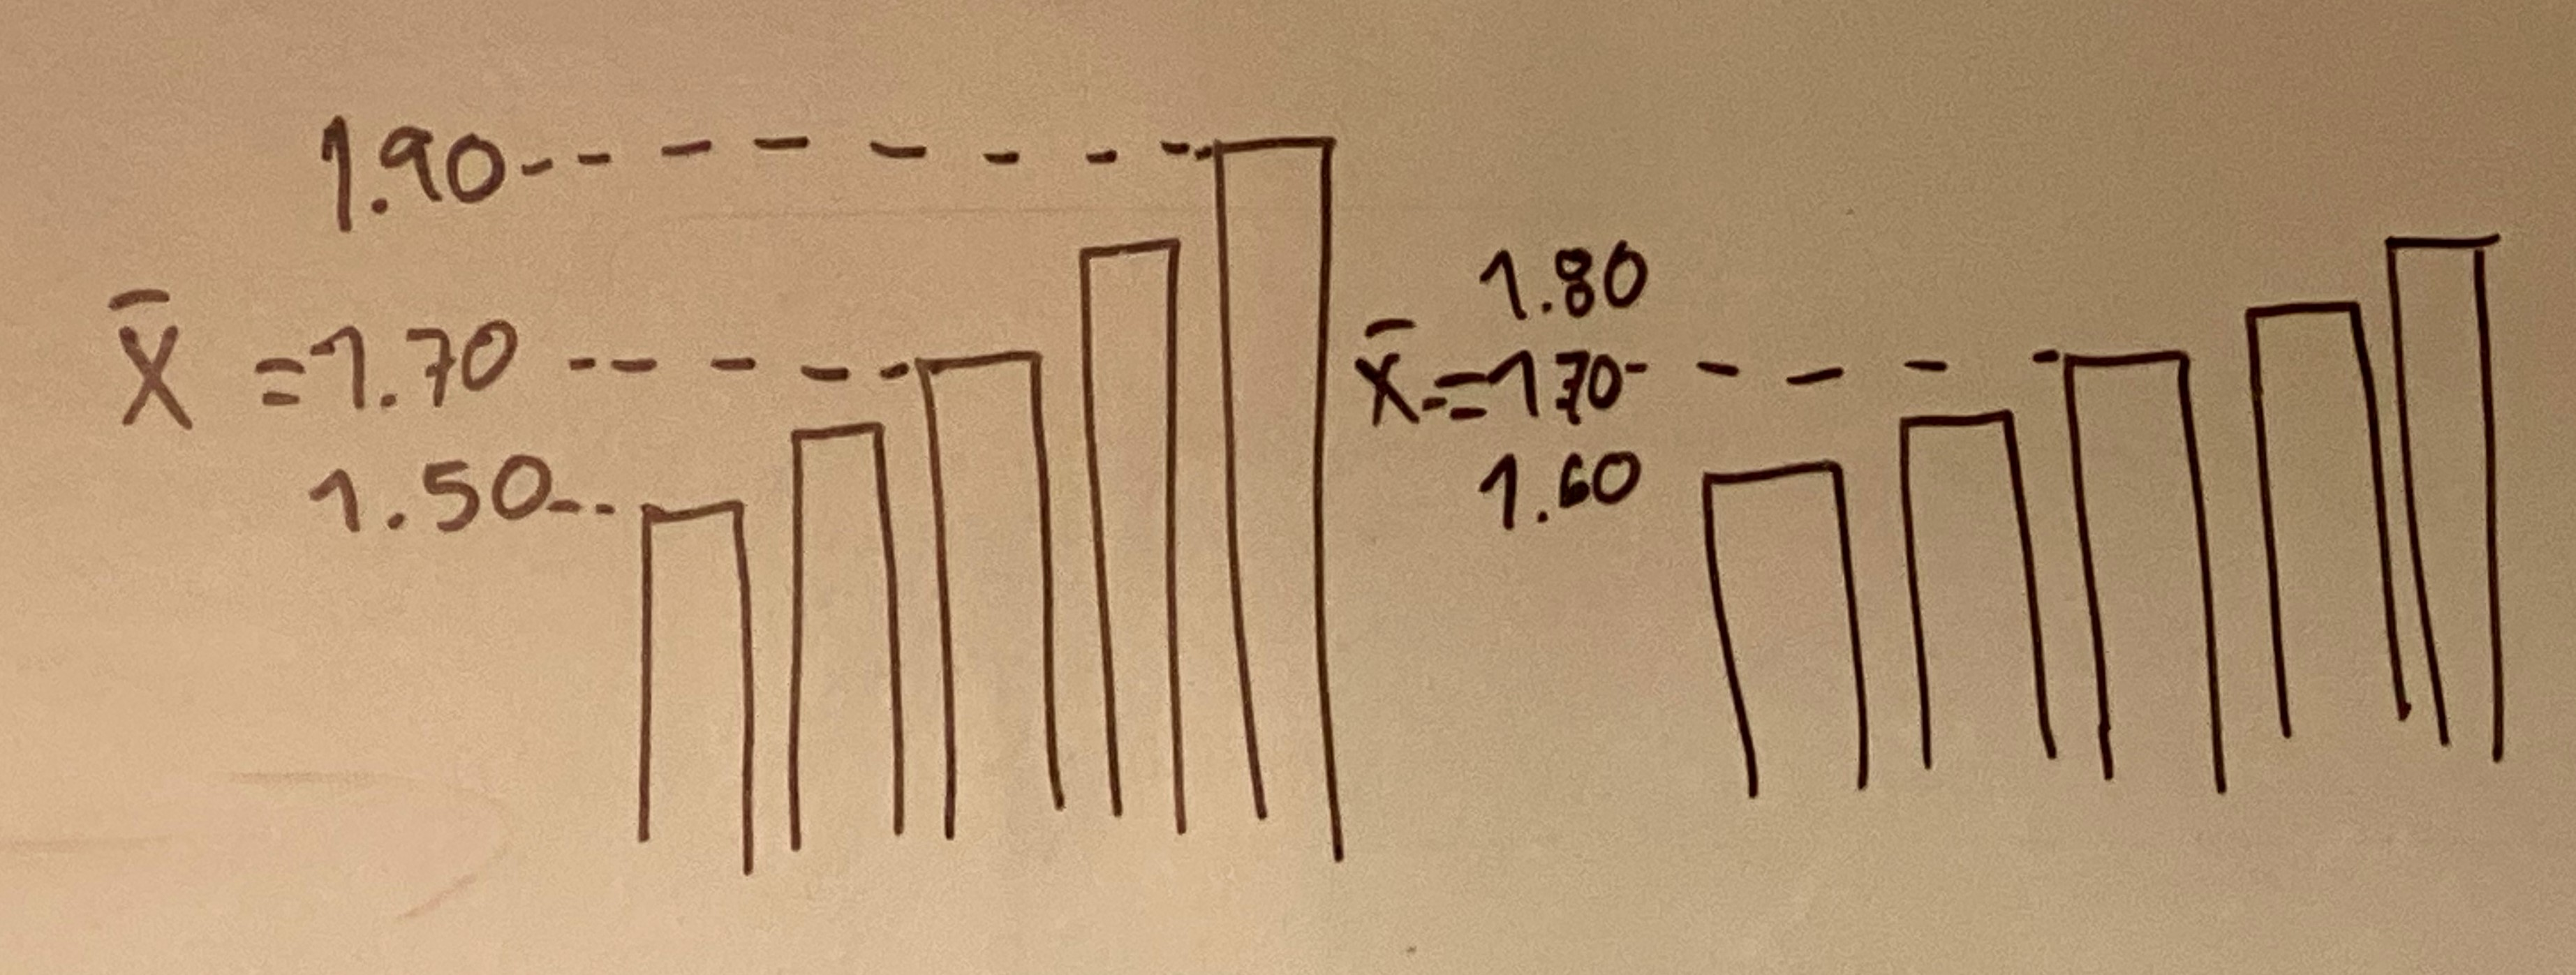
\includegraphics[width=6cm]{./../__Imagenes__/2020-01-16-EstadisticaI.jpeg}
    \caption{Misma media, diferente rango de datos}
    \label{}
\end{figure} 
\begin{itemize}
    \item Los datos están confusos ya que a pesar de tener la misma media los datos varían.
    \item Entonces se introduce el rango que se calcula como:
        \[
            \text{Rango} = \text{Máximo} + \text{Mín}
        \]
\end{itemize}

%%%%%%%%%%%%%%%%%%%%%%%%%%%%%%%%%%%%%%%%%%%%%%%%%%%%%%%%%%%%%%%%%%%%%%%%%%%%%%%%%%%%%%%%%%%%%%%%

\subsubsection{Rango intercuartílico}
La diferencia entre el cuartil tres y el cuartil uno.
\[
   R_{\text{Intercuartílico}} = Q_{3} - Q_{1}
\]
Entre $Q_{3}$ y el $Q_{1}$, \textbf{Nos preguntamos:} ¿qué diferencias hay? es el 50\% de todos los que se parecen entre sí.

%%%%%%%%%%%%%%%%%%%%%%%%%%%%%%%%%%%%%%%%%%%%%%%%%%%%%%%%%%%%%%%%%%%%%%%%%%%%%%%%%%%%%%%%%%%%%%%%
\subsection{Varianza muestral:}
\begin{itemize}
    \item \emph{\textbf{Definición de ``Varianza Muestral":} cuánto varian en promedio los datos respecto a la media.}
    \item Se denota por una $S^2$
    \item \[
        S^2 = \frac{\sum_{i=1}^{n}(X_{i}-\bar{x})}{n-1} 
      \]     
    
    \item Este en el ejemplo esta expresado en centímetros$^2$. 
\end{itemize}

%%%%%%%%%%%%%%%%%%%%%%%%%%%%%%%%%%%%%%%%%%%%%%%%%%%%%%%%%%%%%%%%%%%%%%%%%%%%%%%%%%%%%%%%%%%%%%%%

\subsection{Desviación estándar}
\begin{itemize}
    \item \emph{\textbf{Definición de ``Desviación estándar":} cuánto varían los datos respecto a la media.}
    \item Es la raíz cuadrada de la varianza, se denota por solo $S$.
    \item \[
      \sqrt[]{S^2}  = S = \sqrt[]{ \frac{\sum_{i=1}^{n}(X_{i}-\bar{x})}{n-1} }
    \]
    
    \item En el ejemplo que tenemos está expresado en centímetros.
    \item Desviación estándar significa que en promedio los datos difieren respecto a la media.
    \item Cuando hay una desviación estándar está alta nos dice qué tanto se parecen los datos, qué tan variable es el grupo de datos.
    \item DE: 15 respecto a otra de DV:7, dice que hay más variación en la desviación estándar de 15.
\end{itemize}

%%%%%%%%%%%%%%%%%%%%%%%%%%%%%%%%%%%%%%%%%%%%%%%%%%%%%%%%%%%%%%%%%%%%%%%%%%%%%%%%%%%%%%%%%%%%%%%%
\section{Excel}
\begin{itemize}
    \item Para fijar una celda usar la letra de la columna encerrada por signos de dólar, así: \$E\$56
    \item Para desviación estándar usar fórmula: =DESVEST.M(<TodosLosDatosOriginales>) .
\end{itemize}

%%%%%%%%%%%%%%%%%%%%%%%%%%%%%%%%%%%%%%%%%%%%%%%%%%%%%%%%%%%%%%%%%%%%%%%%%%%%%%%%%%%%%%%%%%%%%%%%

\section{Ejemplo}
\begin{figure}[htbp]
    \centering
    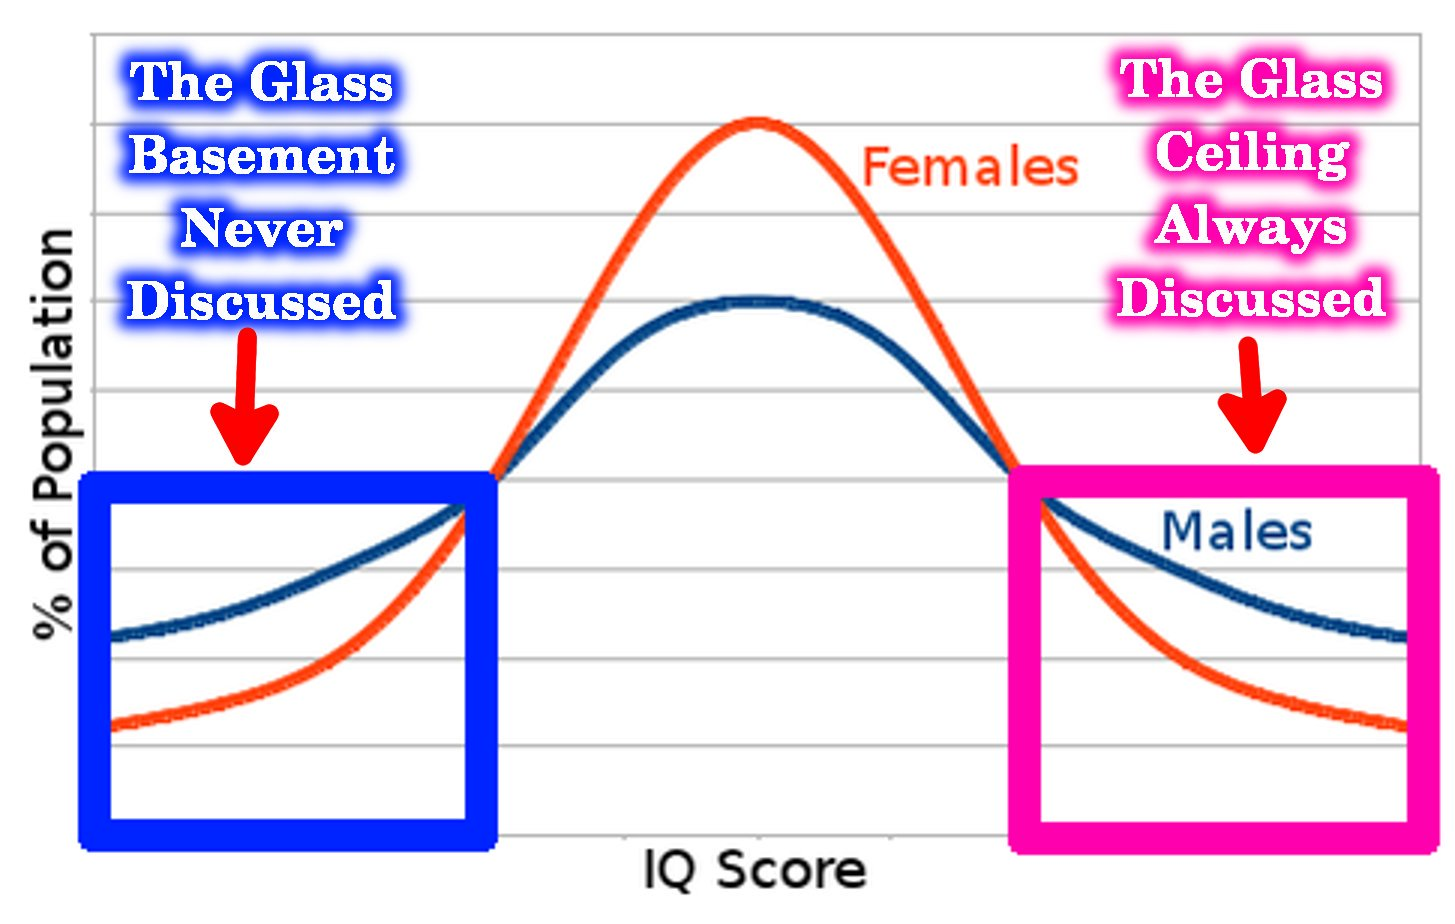
\includegraphics[width=8cm]{../__Imagenes__/2020-01-16-01-ESTADISTICA.jpg}
    \caption{Niveles de IQ entre hombres y mujeres}
    \label{}
\end{figure} 

\begin{itemize}
    \item Las deducciones son que los hombres tienen una desviación estándar mayor.
\end{itemize}
